\documentclass{article}
\usepackage[utf8]{inputenc}
\usepackage[T2A]{fontenc}
\usepackage[russian]{babel}
\usepackage{amsmath}
\usepackage{amssymb}
\usepackage{graphicx}
\usepackage{geometry}
\geometry{a4paper, margin=1in}

\title{Пример генерации таблицы и изображения}
\author{Автоматический генератор LaTeX}
\date{\today}

\begin{document}
\maketitle

\section{Пример таблицы}

Ниже представлена таблица, сгенерированная с помощью функции generate\_table:

\begin{table}[h]
\centering
\begin{tabular}{|c|c|c|}
\hline
Имя & Возраст & Город \\
\hline
Иван & 25 & Москва \\
\hline
Мария & 30 & Санкт-Петербург \\
\hline
Алексей & 22 & Казань \\
\hline
Екатерина & 28 & Новосибирск \\
\hline
\end{tabular}
\caption{Пример таблицы с данными пользователей}
\label{tab:users}
\end{table}

\section{Пример изображения}

Ниже представлено изображение, сгенерированное с помощью функции generate\_image:

\begin{figure}[h]
\centering
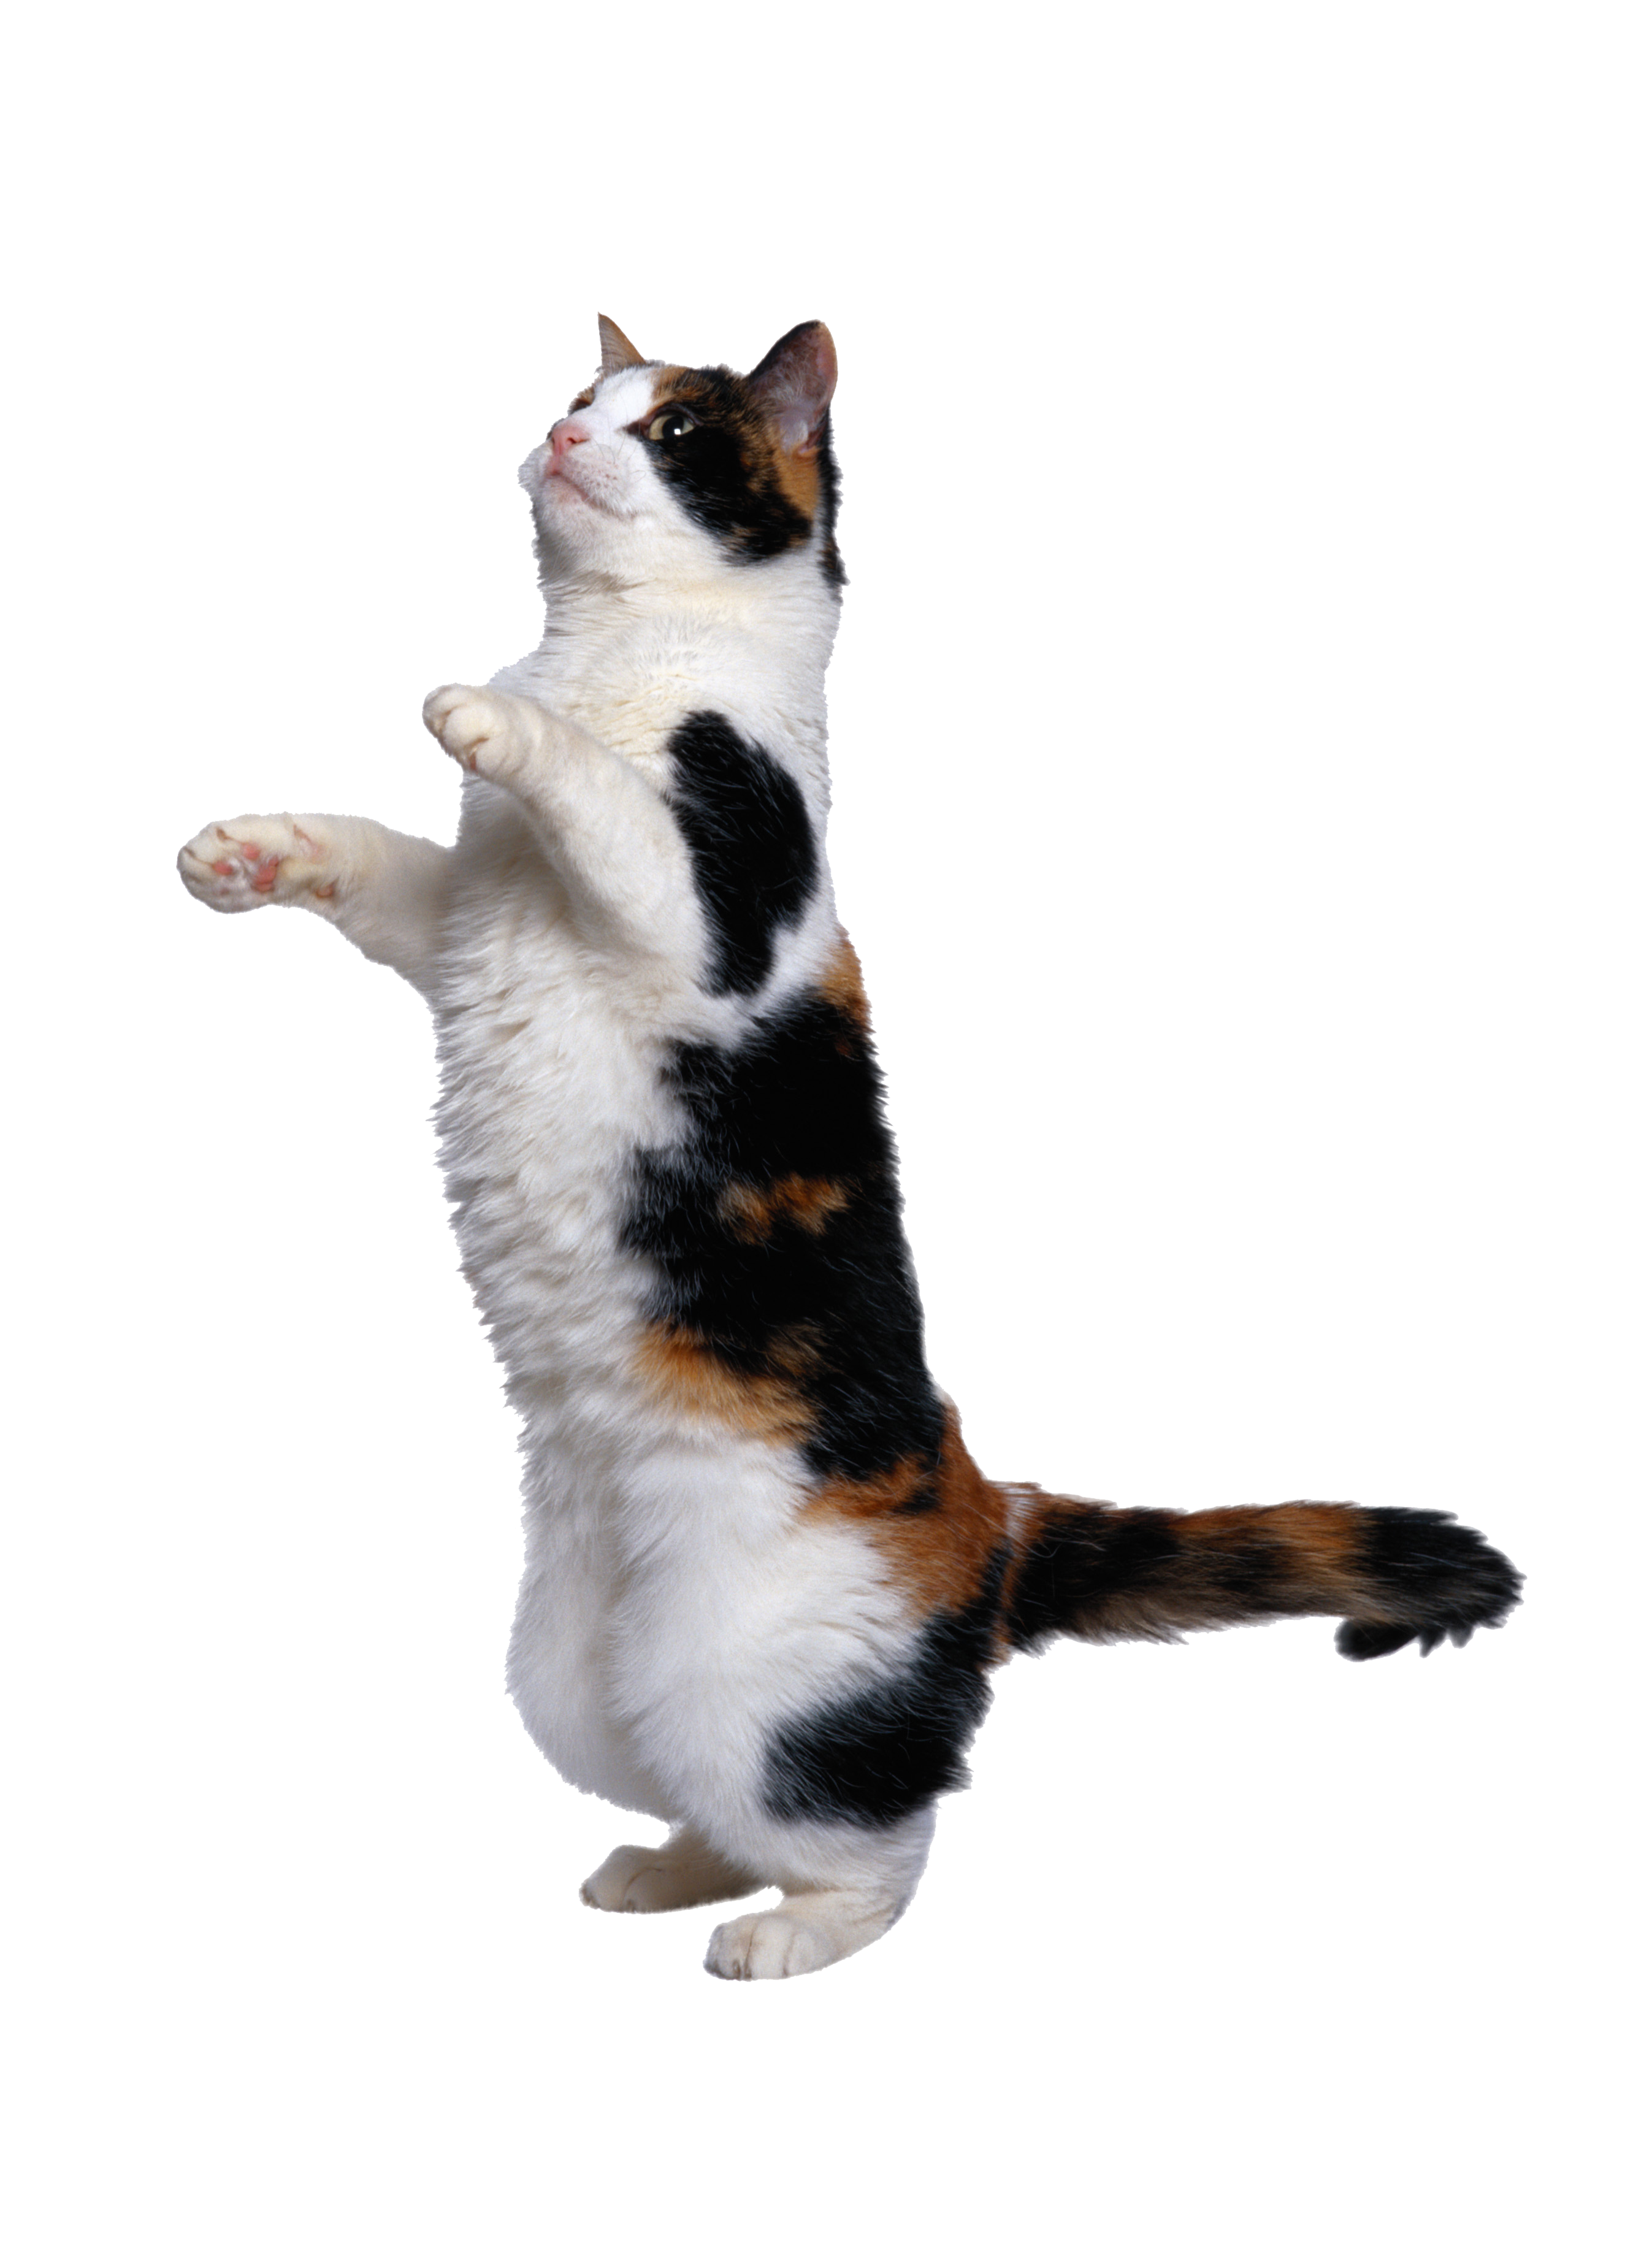
\includegraphics[width=0.8\textwidth]{cat.png}
\caption{Котик}
\label{fig:cat}
\end{figure}
\end{document}